\chapter{Implementation Details}

\section{Case of study 1: Cluster and Honeypot for a DoS attack}
\subsection{Instruments used}
In order to simulate our IoT cluster with the honeypot, we decide to implement a simulation using python. The most important aspect 
to respect when developing a client-server application, like our ioT cluster, it that the servers and the sensors have to able able to exchange data 
between each others. The module sockets present in  the python library allow us to support networking protocols between two or more processes across machines. In this particular case we use TCP sockets, where at one side a process act like a client and on the other side a process act like a server. Also python offer the module selectors that allow us to serve multiple sockets connections. In particular the .select() method allows us to check for I/O completion on more than one socket. So we can call .select() to see which sockets have I/O ready for reading and/or writing.  We also want to underline that with .select()  we’re not able to run concurrently. 
\subsection{ First structure of the IoT cluster}
In our first simulation we decided to implement an high-interaction honeypot and a cluster reported in the figure below.
\begin{figure}[h!]
  \centering
  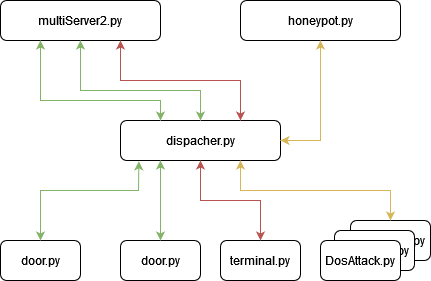
\includegraphics[width = 12cm]{images/HighInterationHoneypot.drawio.png}
  \caption{Our simple IoT cluster with an high-interaction honeypot}
  \label{fig:DosImpl1}
\end{figure}
\FloatBarrier
\noindent
This system help us to underline the difference between the dispacher and the honeypot. In the other section of the report 
where we speak about the implementaions of the Dos honeypot, we mention about IPS and IDS, but it turn out that we need only a system that redirect packets
from the sensors to the honeypot or to the server.  This symple application allow the user to open or close the doors connecetd to the system.
In the nexts subsections we will explain the purpose of every script and how they interact. We would like to remind that on the git repository there is also a tutorial about the use of the first version of the cluster.
\subsection{Door.py}


\subsection{terminal.py}

\subsection{dispacher.py}

\subsection{DosAttack.py}

\subsection{IPS.py}

\subsection{honeypot.py}

\subsection{multiServer2.py}


\begin{figure}[h!]
  \centering
  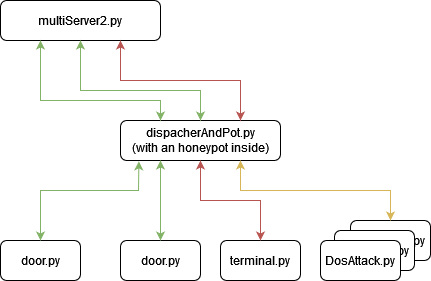
\includegraphics[width = 12cm]{images/lowInterationHoneypot.drawio.png}
  \caption{Our simple IoT cluster with a low-interaction honeypot}
  \label{fig:DosImpl2}
\end{figure}
\FloatBarrier
\noindent







%cancella
This is where you explain what you have implemented and how you have implemented it. Place here all the details that you consider important, organize the chapter in sections and subsections to explain the development and your workflow.\\Given the self-explicative title of the chapter, readers usually skip it. This is ok, because this entire chapter is simply meant to describe the details of your work so that people that are very interested (such as people who have to evaluate your work or people who have to build something more complex starting from what you did) can fully understand what you developed or implemented.\\Don't worry about placing too many details in this chapter, the only essential thing is that you keep everything tidy, without mixing too much information (so make use of sections, subsections, lists, etc.). As usual, pictures are helpful.